% ****** Start of file apssamp.tex ******
%
%   This file is part of the APS files in the REVTeX 4.2 distribution.
%   Version 4.2a of REVTeX, December 2014
%
%   Copyright (c) 2014 The American Physical Society.
%
%   See the REVTeX 4 README file for restrictions and more information.
%
% TeX'ing this file requires that you have AMS-LaTeX 2.0 installed
% as well as the rest of the prerequisites for REVTeX 4.2
%
% See the REVTeX 4 README file
% It also requires running BibTeX. The commands are as follows:
%
%  1)  latex apssamp.tex
%  2)  bibtex apssamp
%  3)  latex apssamp.tex
%  4)  latex apssamp.tex
%
\documentclass[%
 reprint,
%superscriptaddress,
%groupedaddress,
%unsortedaddress,
%runinaddress,
%frontmatterverbose, 
%preprint,
%preprintnumbers,
%nofootinbib,
%nobibnotes,
%bibnotes,
 amsmath,amssymb,
 aps,
%pra,
%prb,
%rmp,
%prstab,
%prstper,
%floatfix,
]{revtex4-2}

\usepackage{graphicx}% Include figure files
\usepackage{dcolumn}% Align table columns on decimal point
\usepackage{bm}% bold math
%\usepackage{hyperref}% add hypertext capabilities
%\usepackage[mathlines]{lineno}% Enable numbering of text and display math
%\linenumbers\relax % Commence numbering lines

%\usepackage[showframe,%Uncomment any one of the following lines to test 
%%scale=0.7, marginratio={1:1, 2:3}, ignoreall,% default settings
%%text={7in,10in},centering,
%%margin=1.5in,
%%total={6.5in,8.75in}, top=1.2in, left=0.9in, includefoot,
%%height=10in,a5paper,hmargin={3cm,0.8in},
%]{geometry}

\begin{document}

\preprint{APS/123-QED}

\title{An Investigation into the Formation of Lenticular Galaxies Through Mergers}% Force line breaks with \\
%\subtitle{ASTR400B Spring 2023}


\author{Carl Ingebretsen}
 \email{carljingebretsen@arizona.edu}
\affiliation{University of Arizona
}

\date{\today}% It is always \today, today,
             %  but any date may be explicitly specified

%\begin{abstract}
%abstract
%\end{abstract}

%\keywords{Suggested keywords}%Use showkeys class option if keyword
                              %display desired
\maketitle

%\tableofcontents

\section{\label{sec:level1}Introduction}
In this project, I will explore the formation of lenticular galaxies as the product of merger remnants. For this goal, I will study the merger of the Milky Way and the Andromeda galaxy with M33 orbiting farther away. A lenticular galaxy is of the type S0. It is a type of galaxy that appears to be intermediate between a spiral galaxy and an elliptical galaxy. The interior regions of the galaxy look like an elliptical galaxy with a large bulge but it is surrounded by a disk of gas. This disk of gas looks like the gas in a spiral galaxy but with little to no evidence of a spiral arm structure. Since this is a usual type of galaxy their origins are contested\citep{Querejeta_2015}.

Because a lenticular galaxy morphologically appears to be a sort of intermediate between spirals and elliptical galaxies, and elliptical galaxies are thought to form as the result of mergers of spiral galaxies, perhaps the lenticular galaxy is an intermediate stage in time after the spirals have merged but before they form a fully elliptical galaxy\citep{Cox_2006}. Elliptical galaxies have little to no cool gas, suggesting that the gas ring of a lenticular galaxy could be left over cool gas of the spirals that hasn’t been heated and ionized yet. The exact formation of elliptical galaxies through mergers is still not well understood. A spiral galaxy has considerable angular momentum while ellipticals generally due not and are dispersion supported\citep{Cox_2006}. How the merger product evolves from being rotationally supported to dispersion supported is of interest.

 An S0 type galaxy's light profile can be described using a Sersic profile of about n=1.0 for the bulge area\citep{Querejeta_2015}. The light profiles of the bulge and disk can be fit separately as seen in a figure provided by Querejeta et al\cite{Querejeta_2015}.
\begin{figure}
    \centering
    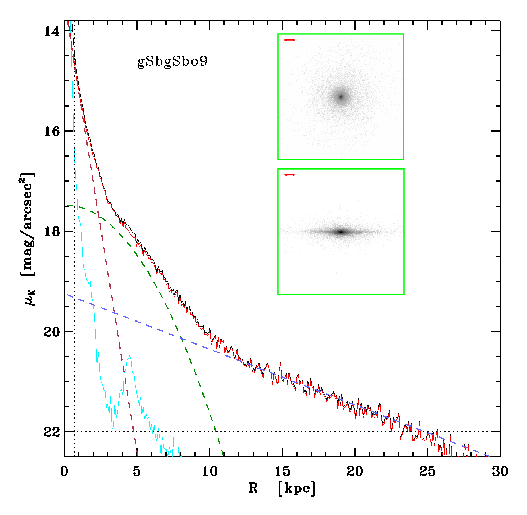
\includegraphics{aa24303-14-fig12.eps}
    \caption{Image of the light profile of a simulated S0 type galaxy. Querejeta et al 2015}
    \label{profile_fig}
\end{figure}
From observational evidence one formation mechanism for S0 galaxies is ram-pressure stripping in galaxy clusters\citep{Querejeta_2015}. However there are many S0 galaxies observed outside confines of clusters, indicating that the ram-pressure stripping can't be the only formation mechanism and hence indicating mergers may be able to result in S0 galaxies.

As of the present, the formation history of lenticular galaxies is still not well understood. Their rotation and dynamics and morphology are apparently intermediate of the spiral and elliptical galaxies. This hints at their origin as merger remnants. It may be possible that the Milky Way and Andromeda merger remnant could at least initially be a lenticular galaxy before evolving further into an elliptical galaxy. This type of evolution can be studied using dynamical simulations, namely n-body simulations. The details of the n-body simulations I will use are elaborated in the paper by van der Marel et. al \citep{van_der_Marel_2012,Sohn_2012}.

\section{Proposal}
The research question that I plan to explore is if the merger remnant of the Milky Way and Andromeda galaxy could be an S0 type galaxy. The origin of the S0 galaxies is of interest since they are an unusual type of galaxy. In connection to this question I will also explore if the remnant of the merger is a slow or fast rotator. This could be a sign of an S0 type galaxy. In addition, if I have time, I would like to plot the velocity dispersion of the remnant as well.

In order to identify if the merger remnant is a lenticular galaxy (S0) it will be necessary to fit the light profile. I will attempt to do this by assuming an average luminosity value for the stellar particles in the simulation and integrating the light within a given radius. This sill result in a graph like that in the introduction\ref{profile_fig}\cite{Querejeta_2015}. I will want to search for a new population of bulge and disk stars if this the remnant is an S0 type. This is illustrated in \ref{fig_2}. The red bulge area should have different dynamics than the disk that is enclosed in the green circle. I will try to explore this also by trying to plot the rotation speed of both components. I will try to search for a large slow rotating bulge and a faster rotating disk. A change in the velocity dispersion between the bulge and disk will also be an indication of the S0 type.
\begin{figure}
    \centering
    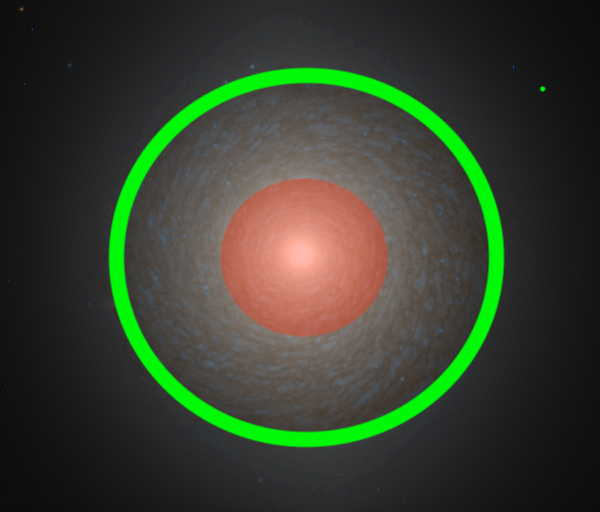
\includegraphics[scale=0.35]{NGC1387_-_hst_10217R850GB475.png}
    \caption{This is an image of an S0 galaxy with color overlays indicating the bulge and disk components.}
    \label{fig_2}
\end{figure}

There is some evidence that the mergers of similar mass large galaxies can produce lenticular galaxies \citep{Querejeta_2015}. However this seems to be a rather tentative result so I don't expect a perfect S0 identification. i will hope for some sign that the tidal tales can orbit to become a disk and hence form an S0 galaxy. I personally expect that S0 galaxies are a short lived phase for a galaxy. It may happen that the merger remnant may initially resemble a S0 type but the disk could disperse and result in a more classical elliptical galaxy at later times in the simulation.

\appendix

% The \nocite command causes all entries in a bibliography to be printed out
% whether or not they are actually referenced in the text. This is appropriate
% for the sample file to show the different styles of references, but authors
% most likely will not want to use it.
\nocite{*}

\bibliography{apssamp}% Produces the bibliography via BibTeX.

\end{document}
%
% ****** End of file apssamp.tex ******
